%%
%% プリアンブル
%%==============================================================================================================================%%
\RequirePackage{fix-cm}
%%
%% ドキュメントクラスとオプションの指定
%%--------------------------------------------------------------------------------------------------------------------%%
\documentclass[10pt,a4paper,disablejfam,dvipdfmx,fleqn,onecolumn,oneside,openany,report]{jsarticle}
%%
%% パッケージの読み込み
%%--------------------------------------------------------------------------------------------------------------------%%
\input{/usr/local/etc/Package}
%%
%% コマンドと環境の定義
%%--------------------------------------------------------------------------------------------------------------------%%
\input{/usr/local/etc/Defines}
%%
%% ページレイアウト設定(A4横組用レイアウト for jsreport)
%%--------------------------------------------------------------------------------------------------------------------%%
\input{/usr/local/etc/Layouts}
%%
%% タイトル・著者名・作成日の設定
%%--------------------------------------------------------------------------------------------------------------------%%
\title{質問回答} \author{姫 伯邑考} \date{2017年01月26日}
%%
%% 本文
%%====================================================================================================================%%
\begin{document}
\maketitle
\begin{itemize}
\item[\ajMaru{3}] 円周上に $\mathrm{A}_{1}$、$\mathrm{A}_{2}$、$\cdots$、$\mathrm{A}_{12}$ の 12 点を等間隔にとり、円に内接する正十二角形を作る。
  これらの 12 点から3点を選んで結び三角形を作るとき、$\mathrm{A}_{1}$ を頂点とする鋭角三角形は \ovalbox{ア} 個できる。
  また、$\mathrm{A}_{1}$、$\mathrm{A}_{3}$ を頂点とする鋭角三角形は \ovalbox{イ} 個でき、$\mathrm{A}_{1}$、$\mathrm{A}_{6}$ を頂点とする鋭角三角形は \ovalbox{ウ} 個できる。
  \begin{solve}
    \begin{itemize}
    \item[ア)] 正十二角形が内接する円の中心を $\mathrm{O}$ とすると、点 $\mathrm{O}$ を通る対角線を1辺とする三角形が直角三角形となるので、点 $\mathrm{A}_{1}$ を頂点として鋭角三角形になるための条件は、
      \begin{center}「線分 $\mathrm{OA}_{7}$ と交わる(端点は含まない)対角線を1辺とする」\end{center}
      である。$\mathrm{OA}_{7}$ と交わる対角線の本数は 10 本なので、$\mathrm{A}_{1}$ を頂点とする鋭角三角形は 10 個。$\cdots$ \ovalbox{ア}

    \item[イ)] $\mathrm{A}_{3}$ から引ける対角線の中で線分 $\mathrm{OA}_{7}$ と交わるものは1本存在する。故に、1個。$\cdots$ \ovalbox{イ}

    \item[ウ)] $\mathrm{A}_{6}$ から引ける対角線の中で線分 $\mathrm{OA}_{7}$ と交わるものは4本存在する。故に、4個。$\cdots$ \ovalbox{ウ}
    \end{itemize}
  \end{solve}
\end{itemize}
\vspc{-5.00pt}\begin{figure}[H]\centering\scalebox{1.00}{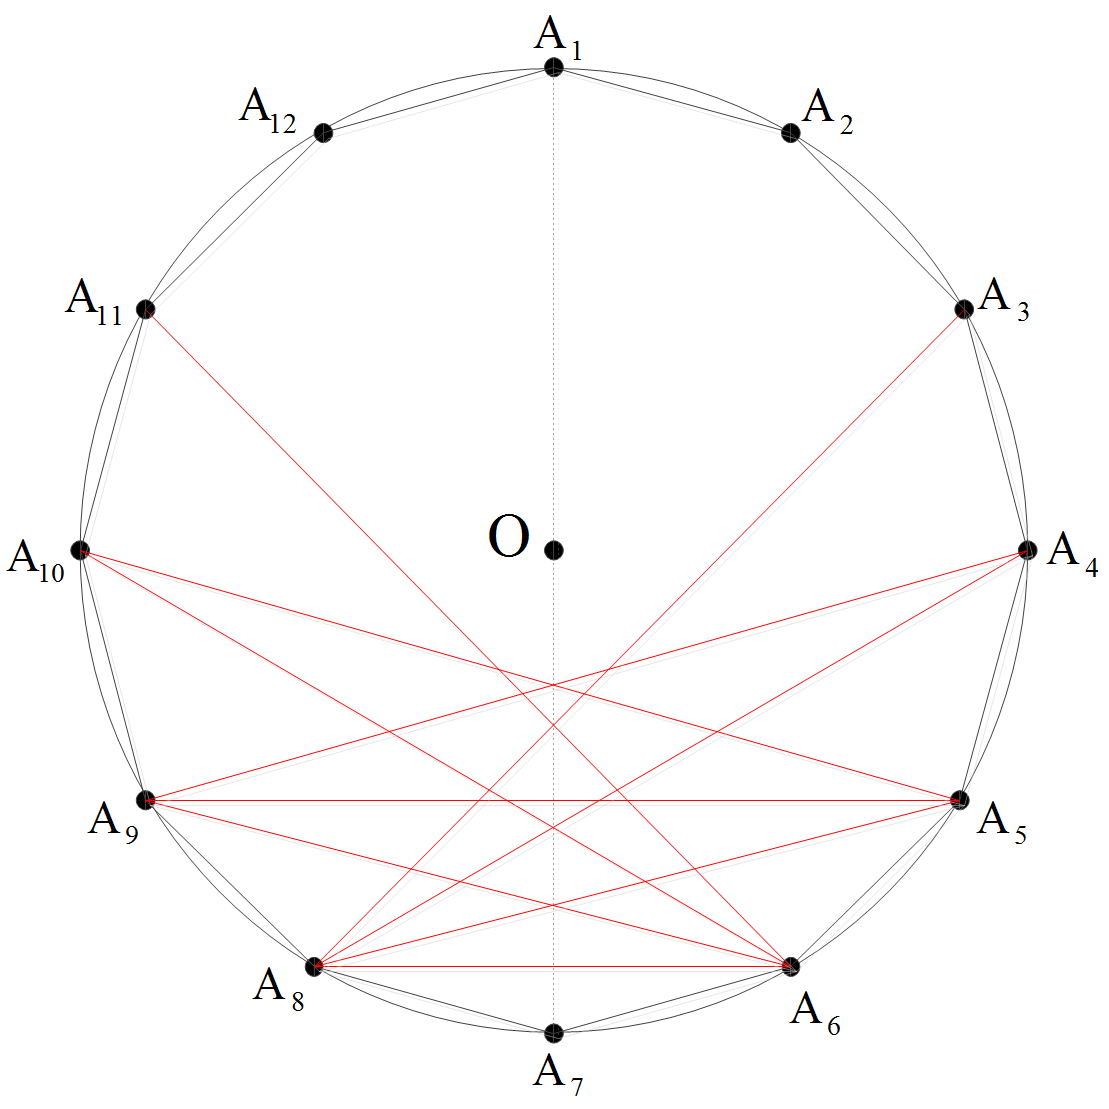
\includegraphics{./Fig/Fig001.PNG}}\end{figure}\vspc{-5.00pt}
\end{document}
